% ============================================================
%  File   : Teoria.tex
%  Capitolo: Richiami Teorici
%  Posizione nel repository: SP/latex/Teoria.tex
% ============================================================

\chapter{Richiami Teorici}

Si richiamano di seguito i fondamenti matematici e fisici che costituiscono la base
del codice CFD sviluppato nel corso.
Le sezioni seguono il filo logico dell'implementazione: dalle equazioni di governo
alla loro discretizzazione, dai flussi numerici all'integrazione temporale,
fino agli strumenti di verifica della convergenza.

% ============================================================
\section{Equazioni di Governo: Eulero 2D}
% ============================================================

Il codice risolve le \textbf{equazioni di Eulero 2D}, che descrivono il moto di un
fluido comprimibile non viscoso.
Nella forma conservativa differenziale:

\begin{equation}
  \parziale{\uvec}{t}
  + \parziale{\fvec}{x}
  + \parziale{\gvec}{y} = \bm{0}
  \label{eq:eulero_diff}
\end{equation}

dove il vettore delle variabili conservative e i vettori dei flussi sono:

\begin{equation}
  \uvec = \begin{pmatrix} \rho E \\ \rho \\ \rho u \\ \rho v \end{pmatrix}, \quad
  \fvec = \begin{pmatrix} u(\rho E + P) \\ \rho u \\ \rho u^2 + P \\ \rho u v \end{pmatrix}, \quad
  \gvec = \begin{pmatrix} v(\rho E + P) \\ \rho v \\ \rho u v \\ \rho v^2 + P \end{pmatrix}
\end{equation}

con $\rho$ densità, $u,\,v$ componenti di velocità, $P$ pressione, $E$ energia totale
specifica.
Il sistema è chiuso dall'equazione di stato dei gas perfetti:

\begin{equation}
  P = (\gamma - 1)\left(\rho E - \tfrac{1}{2}\rho(u^2+v^2)\right), \qquad \gamma = 1.4
\end{equation}

% ============================================================
\section{Adimensionalizzazione}
\label{sec:adim}
% ============================================================

Le equazioni vengono risolte in forma adimensionale.
Scelti $P_{\rm ref} = P^\circ_{\rm in}$ e $T_{\rm ref} = T^\circ_{\rm in}$ come
grandezze di riferimento, le scale caratteristiche derivate sono:
\begin{align*}
  \rho_{\rm ref} &= \frac{P_{\rm ref}}{R T_{\rm ref}}, &
  u_{\rm ref}    &= \sqrt{R T_{\rm ref}}, &
  t_{\rm ref}    &= \frac{L_{\rm ref}}{u_{\rm ref}}
\end{align*}

Una proprietà fondamentale dell'adimensionalizzazione è che le equazioni di Eulero
mantengono la stessa forma: i fattori di scala si elidono, e il codice lavora quindi
con le stesse espressioni indipendentemente dall'adimensionalizzazione scelta.
In pratica, fissando $P^\circ_{\rm in} = 1$ e $T^\circ_{\rm in} = 1$, le condizioni
al contorno e le variabili di campo assumono valori $O(1)$, migliorando il
condizionamento numerico del sistema.

Le variabili adimensionalizzate rilevanti sono:
\begin{align}
  \bar{P} &= \frac{P}{P_{\rm ref}}, &
  \bar{T} &= \frac{T}{T_{\rm ref}}, &
  \bar{\rho} &= \frac{\bar{P}}{\bar{T}}, \\
  \bar{u} &= \frac{u}{u_{\rm ref}} = M \bar{a}, &
  \bar{a} &= \sqrt{\gamma \bar{T}}, &
  \bar{S} &= \gamma \ln \bar{T} - (\gamma-1)\ln \bar{P}
\end{align}

L'entropia adimensionale $\bar{S}$ è particolarmente utile per la validazione: in un
campo di Eulero privo di onde d'urto $\bar{S}$ è conservata lungo le linee di flusso,
quindi ogni deviazione da zero è imputabile all'errore numerico di discretizzazione.

% ============================================================
\section{Discretizzazione a Volumi Finiti}
% ============================================================

Integrando l'equazione~\eqref{eq:eulero_diff} sul volume della cella $\Omega_i$:
\begin{equation}
  \parziale{}{t} \int_{\Omega_i} \uvec \, d\Omega
  + \oint_{\partial\Omega_i} \left(\fvec n_x + \gvec n_y\right) dS = \bm{0}
\end{equation}

Approssimando con il valore medio sulla cella e la somma dei flussi sui lati:
\begin{equation}
  \parziale{\uvec_i}{t} = -\frac{1}{|\Omega_i|}
  \sum_{j \in \mathcal{N}(i)} \Fvec_{ij} \cdot \nhat_{ij} \, l_{ij}
  \label{eq:volumi_finiti}
\end{equation}

dove $\Fvec_{ij}$ è il flusso numerico all'interfaccia tra la cella $i$ e il suo
vicino $j$, $\nhat_{ij}$ la normale uscente da $i$, e $l_{ij}$ la lunghezza
dell'interfaccia.

% ============================================================
\section{Calcolo dei Flussi Numerici}
\label{sec:flussi}
% ============================================================

\subsection{Schema di Lax--Friedrichs Locale}

Lo schema di Lax--Friedrichs è uno schema \emph{centrato} con dissipazione numerica
proporzionale al massimo valore proprio locale:
\begin{equation}
  \Fvec_{ij} = \frac{1}{2}\left[F^L + F^R\right]
               - \frac{\lambda_{\max}}{2}\left(\uvec^R - \uvec^L\right)
\end{equation}
dove $\lambda_{\max} = \max(|\tilde{u}^L|+a^L,\,|\tilde{u}^R|+a^R)$ è la velocità
massima di propagazione e $\tilde{u} = \bm{q}\cdot\nhat$ è la velocità normale
all'interfaccia.

I flussi vengono calcolati nel sistema di riferimento \emph{ruotato} locale
all'interfaccia, sfruttando la matrice di rotazione:
\begin{equation}
  \begin{pmatrix} \tilde{u} \\ \tilde{v} \end{pmatrix} =
  \begin{pmatrix} n_x & n_y \\ -n_y & n_x \end{pmatrix}
  \begin{pmatrix} u \\ v \end{pmatrix}
\end{equation}
I flussi di quantità di moto vengono poi riportati nel sistema globale tramite
la trasposta della stessa matrice (ortogonale: $R^{-1} = R^T$).

\subsection{Schema di Roe (Upwind)}

Lo schema di Roe è un metodo \emph{upwind} che tiene conto della propagazione
direzionale delle onde caratteristiche. Il flusso è:
\begin{equation}
  \Fvec_{ij} = \frac{1}{2}\left[F^L + F^R\right]
               - \frac{1}{2} \sum_{k=1}^{4} |\hat{\lambda}_k| \hat{\alpha}_k \hat{r}_k
\end{equation}
dove $\hat{\lambda}_k$, $\hat{r}_k$, $\hat{\alpha}_k$ sono rispettivamente i valori
propri, i vettori propri destri e le \emph{wave strengths} della matrice Jacobiana
di Roe, costruita con le medie di Roe tra gli stati $L$ e $R$:
\begin{align}
  \sqrt{\hat{\rho}} &= \sqrt{\rho^L\rho^R}, &
  \hat{u} &= \frac{\sqrt{\rho^L}\,u^L + \sqrt{\rho^R}\,u^R}{\sqrt{\rho^L}+\sqrt{\rho^R}}, &
  \hat{H} &= \frac{\sqrt{\rho^L}\,H^L + \sqrt{\rho^R}\,H^R}{\sqrt{\rho^L}+\sqrt{\rho^R}}
\end{align}

Lo schema di Roe è più accurato di Lax--Friedrichs perché è meno dissipativo e
cattura meglio le discontinuità (onde d'urto) e le strutture fini del campo.

\paragraph{Perché serve l'\emph{entropy fix}.}
La dissipazione numerica dello schema di Roe per la $k$-esima onda è proporzionale a
$|\hat{\lambda}_k|$: l'autovalore agisce da coefficiente di dissipazione. Il problema nasce in
corrispondenza dei \textbf{punti sonici} (\emph{sonic points}), dove un autovalore
\textbf{cambia segno} e si annulla ($\hat{\lambda}_k \to 0$), ad esempio quando $u - a$ passa da
negativo a positivo attraversando una transizione sonica ($M=1$). In quel punto la dissipazione
$|\hat{\lambda}_k| \to 0$ \textbf{svanisce}: lo schema, costruito risolvendo \emph{esattamente} un
problema di Riemann linearizzato, non distingue più tra una compressione (urto, fisicamente
ammesso) e una \textbf{espansione}; può così ammettere un'\textbf{espansione discontinua}
(\emph{expansion shock}), soluzione matematicamente valida ma \textbf{non fisica} perché
viola la condizione di entropia. È questa la causa delle cosiddette \emph{stagnation-point} e
\emph{sonic-point anomalies}.

\paragraph{Correzione di Harten.}
La \textit{entropy fix} di Harten elimina il problema imponendo una \textbf{dissipazione minima}
anche dove l'autovalore si annulla: si sostituisce $|\hat{\lambda}_k|$ con una funzione
$\Psi(\hat{\lambda}_k)$ regolarizzata che non scende mai sotto una piccola soglia $\delta$:
\begin{equation}
  \Psi(\hat{\lambda}_k) =
  \begin{cases}
    |\hat{\lambda}_k| & \text{se } |\hat{\lambda}_k| \ge \delta \\[4pt]
    \dfrac{\hat{\lambda}_k^2 + \delta^2}{2\,\delta} & \text{se } |\hat{\lambda}_k| < \delta
  \end{cases}
\end{equation}
dove $\delta$ è una piccola frazione della velocità caratteristica locale (tipicamente
$\delta = \epsilon(|\hat u| + \hat a)$ con $\epsilon \sim 0.1$). In pratica si "arrotonda" il
valore assoluto vicino allo zero, garantendo una dissipazione residua che \textbf{impedisce le
espansioni non fisiche} senza degradare l'accuratezza lontano dai punti sonici.

% ============================================================
\section{Integrazione Temporale}
% ============================================================

L'integrazione nel tempo è esplicita con schema di Eulero in avanti:
\begin{equation}
  \uvec_i^{k+1} = \uvec_i^k + \dt \parziale{\uvec_i}{t}^k
\end{equation}

Il passo temporale $\dt$ è calcolato ad ogni iterazione imponendo la condizione CFL:
\begin{equation}
  \dt = \text{CFL} \cdot \min_i \frac{\sqrt{|\Omega_i|}}{\lambda_{\max,i}}
  \label{eq:cfl}
\end{equation}

dove $\lambda_{\max,i} = |\bm{q}_i| + a_i$ è la velocità di propagazione massima
nella cella $i$.
Il fattore $\sqrt{|\Omega_i|}$ approssima la dimensione caratteristica della cella
in 2D ($h \propto \sqrt{A}$, analogamente a $h \propto \sqrt[3]{V}$ in 3D).

% ============================================================
\section{Condizioni al Contorno}
% ============================================================

Le condizioni al contorno dipendono dalla direzione del flusso e dal regime locale:
\begin{itemize}
  \item \textbf{Inlet subsonico}: si impongono $T^\circ_{\rm in}$, $P^\circ_{\rm in}$,
    $\alpha_{\rm in}$; il numero di Mach è estrapolato dall'interno.
  \item \textbf{Inlet supersonico}: si impongono tutte e quattro le variabili
    conservative (flusso completamente entrante, nessuna caratteristica uscente).
  \item \textbf{Outlet subsonico}: si impone la pressione statica $P_{\rm exit}$;
    le altre tre variabili sono estrapolate dall'interno.
  \item \textbf{Outlet supersonico}: tutte le variabili sono estrapolate
    (nessuna caratteristica entrante).
  \item \textbf{Parete solida}: condizione di impermeabilità ($\bm{q}\cdot\nhat = 0$),
    implementata con una cella specchio che annulla la componente normale della velocità.
\end{itemize}

% ============================================================
\section{Analisi di Convergenza della Griglia}

\subsection{Valutazione dell'Ordine di Convergenza con la Norma $L_2$ dell'Entropia}

Per quantificare l'errore numerico di discretizzazione si utilizza la norma $L_2$ (valore quadratico medio) dell'entropia adimensionale $\bar{S}$. In un campo di moto Euleriano privo di onde d'urto (flusso puramente subsonico), l'entropia deve conservarsi costante lungo le linee di corrente. Assumendo un ingresso isentropico, il valore analitico esatto dell'entropia nel dominio è ovunque nullo ($S_{\rm esatto} = 0$). 

Qualsiasi deviazione da questo valore misurata nella soluzione numerica rappresenta puramente l'errore di troncamento dovuto alla discretizzazione spaziale. La norma $L_2$ valuta questo errore integralmente su tutto il dominio:
\begin{equation}
  \|\bar{S}\|_2 = \sqrt{\frac{\displaystyle\sum_i \bar{S}_i^2 \cdot |\Omega_i|}
                              {\displaystyle\sum_i |\Omega_i|}}
  \label{eq:norma_entropia}
\end{equation}

Assumendo che l'errore segua un andamento asintotico del tipo $E = k \cdot h^p$, dove $h$ è la dimensione caratteristica della griglia e $p$ è l'ordine di convergenza effettivo, ci si aspetta che $\|\bar{S}\|_2 \to 0$ per $h \to 0$. Calcolando $\|\bar{S}\|_2$ su griglie via via più fitte, la pendenza della curva in un grafico log-log fornisce il valore dell'ordine di convergenza spaziale $p$.

\paragraph{Ambito di validità.}
È importante sottolineare che questo approccio alla valutazione dell'ordine di convergenza, basato sulla \emph{conoscenza analitica} della soluzione esatta ($S_{\rm esatto}=0$), è applicabile \textbf{esclusivamente al caso del bump}. Esso richiede infatti che siano simultaneamente verificate tre condizioni: il flusso deve essere \textbf{subsonico e privo di onde d'urto} (così che l'entropia si conservi e sia ovunque nulla), e il solutore deve essere \textbf{inviscido} (le equazioni di Eulero non includono perdite di strato limite o effetti viscosi che genererebbero entropia fisica). Solo in questo scenario qualsiasi deviazione di $\bar{S}$ da zero è imputabile unicamente all'errore numerico, rendendo la norma $L_2$ dell'entropia un misuratore diretto dell'errore di discretizzazione. Nei casi con urti (ad esempio la presa a doppia rampa) l'entropia esatta \emph{non} è più nulla — viene prodotta fisicamente attraverso gli urti — e questa tecnica non è utilizzabile: in tali casi si ricorre all'estrapolazione di Richardson (Sez.~\ref{subsec:richardson}).

\subsection{Estrapolazione di Richardson}
\label{subsec:richardson}

L'estrapolazione di Richardson è una tecnica che permette di stimare il valore esatto di una grandezza (o un errore residuo) combinando i risultati ottenuti su griglie con livelli di raffinamento diversi. Può essere applicata in due modalità.

\paragraph{1. Ordine assunto pari a quello teorico.}
Se si ha forte confidenza che il metodo numerico stia operando nella regione asintotica, si può ipotizzare che l'ordine effettivo $p$ sia pari all'ordine formale teorico dello schema (ad esempio, $p=1$ per Lax-Friedrichs o Roe al primo ordine). Eseguendo due simulazioni con lunghezze caratteristiche $h_1$ e $h_2 = r h_1$ (con $r > 1$ \emph{rapporto di diradamento}), l'errore si esprime come:
\begin{equation}
  r = \frac{h_2}{h_1} > 1
  \label{eq:rapporto_diradamento}
\end{equation}
Il rapporto di diradamento quantifica di quanto una griglia è più grossolana dell'altra: essendo $r>1$ si ha $h_2 > h_1$, ovvero la griglia con passo $h_2$ è \textbf{più rada} (celle più grandi) rispetto a quella con passo $h_1$, che è la \textbf{più fitta}. Il valore tipicamente adottato è $r=2$, corrispondente al dimezzamento del numero di nodi per direzione fra un livello e il successivo.
\begin{equation}
  \begin{cases}
    E_1 = u_{h_1} - u_{\rm esatto} = k \cdot h_1^p \\
    E_2 = u_{h_2} - u_{\rm esatto} = k \cdot (r h_1)^p
  \end{cases}
\end{equation}
Risolvendo il sistema per l'incognita $u_{\rm esatto}$, si ottiene la formula di estrapolazione:
\begin{equation}
  u_{\rm esatto} \approx \frac{r^p u_{h_1} - u_{h_2}}{r^p - 1}
\end{equation}

\paragraph{2. Ordine empirico (effettivo).}
Se non si conosce a priori l'ordine reale del metodo sulla specifica griglia (ad esempio a causa di effetti di bordo o mesh non sufficientemente fitta), l'ordine $p$ diventa un'incognita. È necessario introdurre una terza simulazione per chiudere il sistema. Date tre griglie con passo $h$, $2h$ e $4h$ (rapporto costante $r=2$), si valuta prima l'ordine effettivo $p$:
\begin{equation}
  p = \frac{\ln\!\left(\dfrac{u_{4h}-u_{2h}}{u_{2h}-u_h}\right)}{\ln 2}
\end{equation}
Una volta trovato $p$, lo si sostituisce nella formula dell'estrapolazione per ricavare la stima accurata della soluzione esatta:
\begin{equation}
  u_{\rm esatto} \approx u_h + \frac{u_{2h}-u_h}{2^p - 1}
\end{equation}

\paragraph{Quando usare l'ordine teorico.} L'ipotesi $p = p_{\rm teorico}$ è lecita
\emph{solo} se si ha confidenza di operare nella \textbf{regione asintotica}, ossia con griglie
sufficientemente fitte da rendere il termine dominante $k\,h^p$ molto maggiore dei termini di
ordine superiore nello sviluppo dell'errore. Su griglie grossolane ciò non accade: l'ordine
\emph{osservato} differisce da quello formale (tipicamente risulta \textbf{inferiore} per la
dissipazione numerica e gli effetti di bordo, ma può apparire anche superiore, come nel caso
della presa a doppia rampa con Roe, dove $p_{\rm eff}\approx1.46$). La Figura~\ref{fig:ordine_convergenza}
illustra qualitativamente l'andamento dell'ordine osservato in funzione del raffinamento: lontano
dalla regione asintotica l'ordine è distante dal valore teorico, e solo infittendo la griglia vi
si avvicina. Lo schema di Roe (upwind, meno dissipativo) converge al valore formale più
rapidamente di Lax--Friedrichs.

\begin{figure}[H]
  \centering
  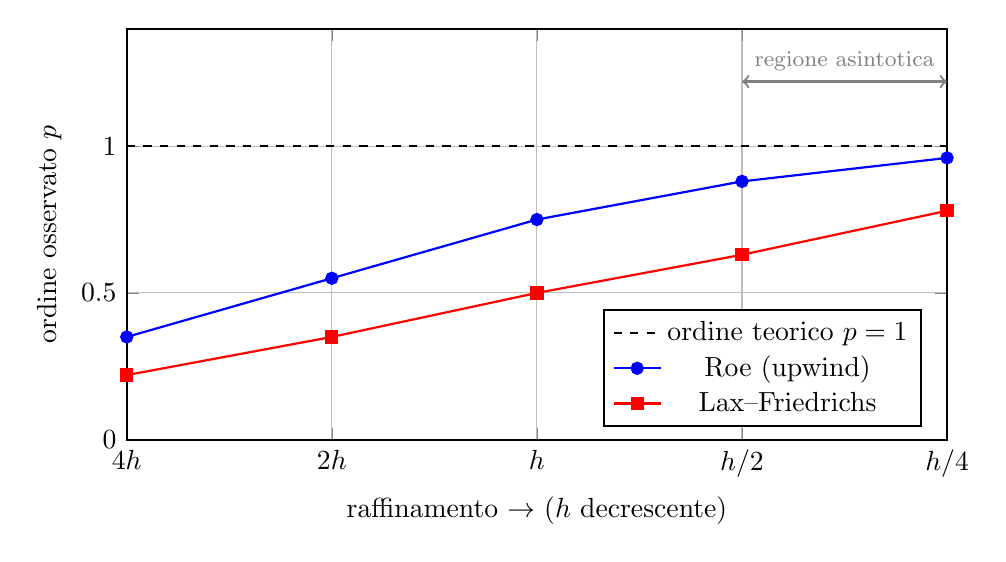
\begin{tikzpicture}
    \begin{axis}[
        width=12cm, height=6.8cm,
        xlabel={raffinamento $\rightarrow$ ($h$ decrescente)},
        ylabel={ordine osservato $p$},
        xmin=0, xmax=4, ymin=0, ymax=1.4,
        xtick={0,1,2,3,4},
        xticklabels={$4h$,$2h$,$h$,$h/2$,$h/4$},
        legend pos=south east, grid=both, thick]
      \addplot[black, dashed, domain=0:4] {1.0};
      \addlegendentry{ordine teorico $p=1$}
      \addplot[blue, mark=*] coordinates {(0,0.35)(1,0.55)(2,0.75)(3,0.88)(4,0.96)};
      \addlegendentry{Roe (upwind)}
      \addplot[red, mark=square*] coordinates {(0,0.22)(1,0.35)(2,0.50)(3,0.63)(4,0.78)};
      \addlegendentry{Lax--Friedrichs}
      \draw[gray, <->] (axis cs:3,1.22) -- (axis cs:4,1.22)
        node[midway, above, font=\footnotesize]{regione asintotica};
    \end{axis}
  \end{tikzpicture}
  \caption{Andamento qualitativo dell'ordine di convergenza osservato in funzione del livello di
           raffinamento. Per griglie grossolane l'ordine effettivo è inferiore a quello teorico
           ($p=1$, tratteggiato); solo entrando nella regione asintotica l'ordine tende al valore
           formale. Lo schema di Roe vi si avvicina più rapidamente di Lax--Friedrichs, coerentemente
           con la sua minore dissipazione numerica.}
  \label{fig:ordine_convergenza}
\end{figure}

Il \textbf{Grid Convergence Index} (GCI) fornisce infine una stima conservativa dell'incertezza numerica associata alla discretizzazione:
\begin{equation}
  \text{GCI} = F_s \cdot |u_h - u_{\rm esatto}|, \qquad F_s = 3 \quad \text{(fattore di sicurezza)}
\end{equation}